\phantomsection
\section{集合}
\phantomsection
\subsection{集合の定義と表記法}

\phantomsection
\subsubsection{集合の定義}

現代数学の基礎をなす概念に「集合」や「写像」がある.まず「集合」からみていこう.
\phantomsection
\begin{definition}{集合}{集合}
  もののあつまりを\emph{集合}\index{しゅうごう@集合}という\footnote{公理的集合論の立場では,集合とは「無定義語」であるが,ここで詳しくは触れない.}.集合を構成するものを\emph{元}\index{げん@元}または\emph{要素}\index{ようそ@要素}といい,集合$A$の元が$a$であることを$a \in A$,$A \ni a$などと表す.
\end{definition}

集合に関して,いくつか注意点を挙げよう.

\begin{itemize}
  \item 集合では書き並べる順序が重要でないため,例えば $\{1, 2, 3\} = \{3, 2, 1\}$である.
  \item 同じ要素が重複して含まれていても,1つの要素として扱われるため,例えば$\{1, 1, 2, 2, 2, 3\} = \{1, 2, 3\}$である.
  \item 集合の要素には,種類が異なるものを同時に含めることができる.例えば,$\{4, \{3\}\}$では,$4$は数であり,$\{3\}$は集合であるが,集合としての資格がある.
\end{itemize}

「ある集合の要素を部分的に含んでいる集合」を考えることは,数学において重要な意義を持つ.
といっても,現段階で部分集合のイメージを掴むことは難しいので,まず定義を確認して,部分集合の具体的な例はのちほど紹介することにする.

\begin{definition}{集合の相等}{集合の相等}
  集合$A$,$B$のすべての要素が一致しているとき,$A$と$B$は\emph{相等}\index{そうとう@相等}であるといい,これを
  \[
    A = B
  \]
  と表す.

  また,集合$A$と$B$が相等でないとき,
  \[
    A \ne B
  \]
  と表す.
\end{definition}

\begin{mycolumn}
  \deref{集合の相等}を考える意義がぴんとこない読者もいるかもしれない.
  だが,たとえば$\pi$,$\int_{0}^{1} \frac{4}{1+x^2} \, dx$,$4 \sum_{n=0}^{\infty} \frac{(-1)^n}{2n+1}$は異なる表現であるが,すべて円周率を表している.
  このような例からわかるように,「相等」を考えることは数学的な主張を正確に表現するために重要なことなのだ.
\end{mycolumn}

\phantomsection
\begin{definition}{部分集合}{部分集合}
  集合$A$の要素がすべて集合$B$の要素でもあるとき,$A$は$B$の\emph{部分集合}\index{ぶぶんしゅうごう@部分集合}であるといい,これを
  \[
    A \subset B,\quad B \supset A
  \]
  などと表す\footnote{このことを$ A \subseteq B$,$B \supseteq A$とかくこともある.一般に,$A \subset B$,$ B \supset A$と書いた場合には$A=B$の場合を含んで意味をとる.}.
\end{definition}

\begin{definition}{真部分集合}{真部分集合}
  集合$A$の要素がすべて集合$B$の要素であり,なおかつ$A \ne B$であるとき,$A$は$B$の\emph{真部分集合}\index{しんぶぶんしゅうごう@真部分集合}であるといい,これを
  \[
    A \subsetneq B,\quad B \supsetneq A
  \]
  などと表す.
\end{definition}

\phantomsection
\subsubsection{集合の表記}

数学を勉強する上で,よく使う集合には固有の記号を与える場合が多い.以下ではよく使う集合の例を挙げよう.

\begin{shadebox}
  よく使う集合
  \begin{itemize}
    \item $\mathbb{R}$は実数全体の集合を表している.Real numberの頭文字をとった.
    \item $\mathbb{N}=\{0,1,2,\cdots \}$は自然数全体の集合を表している.Natural number の頭文字をとった.
    \item $\mathbb{C}=\{ a+bi \mid a,b \in \mathbb{R}\}$は複素数全体の集合を表している.Complex number の頭文字をとった.
    \item $\mathbb{Z}=\{0, \pm 1 , \pm 2 , \cdots\}$は整数全体の集合を表している.Zはドイツ語由来である,
    \item $\mathbb{Q}=\{ a/b \mid   a,b \in \mathbb{Z},b \ne 0 \}$は有理数全体の集合を表している.「商」を表すイタリア語由来である.
  \end{itemize}
\end{shadebox}


\begin{shadebox}
  数を表す集合以外にも,固有の表記が与えられている集合が存在する.
  \begin{itemize}
    \item $\varnothing$ \footnote{空集合は$\emptyset$と表記することもある.ギリシャ文字の$\phi$で代用されることもあるが,本来の空集合の記号はノルウェー語由来である.}は要素を一つも持たない集合,すなわち\emph{空集合}\index{くうしゅうごう@空集合}を表している.
    \item $\mathcal{P}(A)$は集合$A$のすべての部分集合からなる集合,すなわち\emph{べき集合}\index{べきしゅうごう@べき集合}を表している.
  \end{itemize}
\end{shadebox}



\phantomsection
\begin{example}{}{}
  \[
    x \in \mathbb{Q}
  \]
  と書くことで,$x$は有理数であることを表す.
\end{example}

\phantomsection
\begin{example}{}{}
  \[
    \mathbb{R} \subset \mathbb{C}
  \]
  である.つまり,実数全体の集合は複素数全体の集合の部分集合である.
\end{example}

\phantomsection
\begin{example}{}{}
  $A$を集合とするとき,
  \[
    \varnothing  \subset A
  \]
  である.つまり,空集合は全ての集合の部分集合である.
\end{example}

\phantomsection
\begin{example}{べき集合}{べき集合}
  $A=\{ 1, 2\}$とすると,
  \[
    \mathcal{P}(A) = \{ \varnothing, \{1\}, \{2\}, \{1, 2\}\}
  \]
  である.
\end{example}



集合の表記は文脈により省略されることがある.たとえば,以下のような問題があったとする.
\begin{quotation}
  2次方程式
  \[
    x^2 - 3x -4 =0
  \]
  を解け.
\end{quotation}
$x$が属する全体集合は定められていないが,この場合だと「$x \in \mathbb{C}$」とされることが多い.
よってこの方程式の解は$x = -1 , 4$とする場合が多い.
だが,もちろん$ x \in \mathbb{N}$とするなら,$ -1 \notin \mathbb{N}$なので,この場合の解は$ x= 4$のみである.
ただ,$x$が属する全体集合は,文脈でわかったり明記されている場合が多いので,あまり心配はいらないと筆者は考える.


また,集合はしばしば条件を用いて記述される.

\begin{description}
  \item[外延的記法\index{がいえんてききほう@外延的記法}(列挙形式)] \mbox{} \\
        $\{ a, b, c \}$のように要素を列挙して表す.
  \item[内包的記法\index{ないほうてききほう@内包的記法}(条件形式)] \mbox{} \\
        $\{ x \in \mathbb{N} \mid x \leq 5 \}$のように条件を用いて表す.
\end{description}


\phantomsection
\begin{example}{集合の表記}{集合の表記}
  \[
    \{ 1,2,3 \} = \{ n \in \mathbb{N} \mid  n^2 -4n +3 \leqq 0 \}
  \]
\end{example}

\phantomsection
\subsection{集合の演算}

\subsubsection{共通部分・和集合・差集合・補集合}
集合に対して,以下のような演算を定義することができる.

\phantomsection
\begin{definition}{共通部分・和集合・差集合・補集合}{共通部分・和集合・差集合・補集合}
  $A$と$B$を集合とするとき,以下の定義をする.
  \begin{description}
    \item[共通部分\index{きょうつうぶぶん@共通部分}] \mbox{}\\
          $A$と$B$の両方に属する要素全体の集合を$A \cap B$と表す.これを``$A$ intersection $B$''と読む.
    \item[和集合\index{わしゅうごう@和集合}] \mbox{} \\
          $A$または$B$のいずれかに属する要素全体の集合を$A \cup B$と表す.これを``$A$ union $B$''と読む.
    \item[差集合\index{さしゅうごう@差集合}]\mbox{}\\
          $A$の要素で$B$に属さないもの全体の集合を$A \setminus B$と表す.
    \item[補集合\index{ほしゅうごう@補集合}] \mbox{}\\
          全体集合$X$に対して,$X \setminus A$は$A$の補集合であり,$A^c$と表す.これを``$A$ complement''と読む.
  \end{description}
\end{definition}


\begin{figure}[ht]
  \centering
  \begin{minipage}{0.45\linewidth}
    \centering
    % A∩B のベン図
    \scalebox{0.9}{
      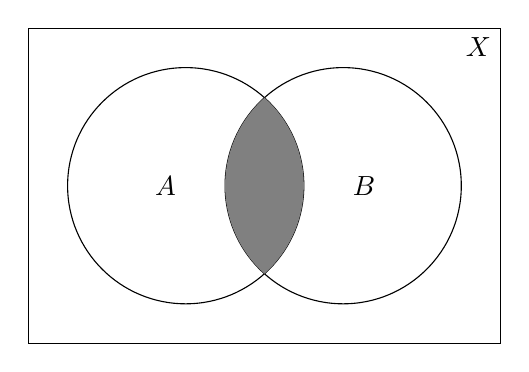
\begin{tikzpicture}
        % 全体集合の長方形
        \draw (0,0) rectangle (6,4) node[below left] {$X$};
        % 集合Aの円
        \draw (2,2) circle (1.5) node[left] {$A$};
        % 集合Bの円
        \draw (4,2) circle (1.5) node[right] {$B$};
        % 共通部分を塗りつぶす
        \begin{scope}
          \clip (2,2) circle (1.5);
          \fill[gray] (4,2) circle (1.5);
        \end{scope}
      \end{tikzpicture}
    }
    \caption{$A \cap B$ のベン図}
  \end{minipage}
  \hfill
  \begin{minipage}{0.45\linewidth}
    \centering
    % A∪B のベン図
    \scalebox{0.9}{
      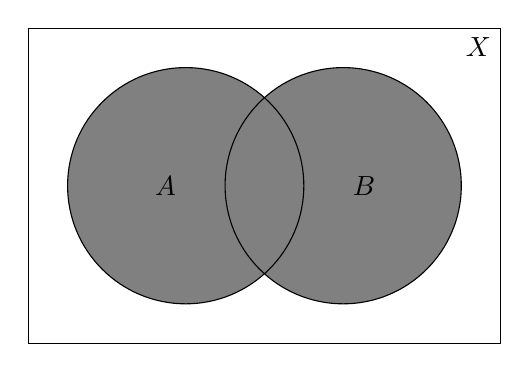
\begin{tikzpicture}
        % 全体集合の長方形
        \draw (0,0) rectangle (6,4) node[below left] {$X$};
        % 集合Aの円を塗りつぶす
        \fill[gray] (2,2) circle (1.5);
        % 集合Bの円を塗りつぶす
        \fill[gray] (4,2) circle (1.5);
        % 集合Aの円の輪郭
        \draw (2,2) circle (1.5) node[left] {$A$};
        % 集合Bの円の輪郭
        \draw (4,2) circle (1.5) node[right] {$B$};
      \end{tikzpicture}
    }
    \caption{$A \cup B$ のベン図}
  \end{minipage}

  \vspace{2mm}

  \begin{minipage}{0.45\linewidth}
    \centering
    % A - B のベン図
    \scalebox{0.9}{
      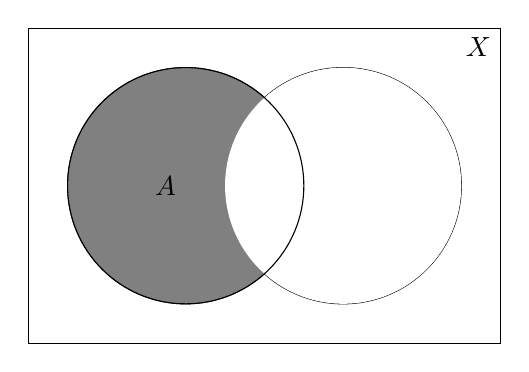
\begin{tikzpicture}
        % 全体集合の長方形
        \draw (0,0) rectangle (6,4) node[below left] {$X$};
        % 集合Aの円
        \draw (2,2) circle (1.5) node[left] {$A$};
        % 集合Bの円
        \draw (4,2) circle (1.5) node[right] {$B$};
        % A - B を塗りつぶす
        \begin{scope}
          \clip (2,2) circle (1.5);
          \fill[gray] (0,0) rectangle (6,4);
        \end{scope}
        \begin{scope}
          \clip (4,2) circle (1.5);
          \fill[white] (0,0) rectangle (6,4);
        \end{scope}
        % 集合Aの円の輪郭
        \draw (2,2) circle (1.5) node[left] {$A$};
      \end{tikzpicture}
    }
    \caption{$A \setminus B$ のベン図}
  \end{minipage}
  \hfill
  \begin{minipage}{0.45\linewidth}
    \centering
    % A^c のベン図
    \scalebox{0.9}{
      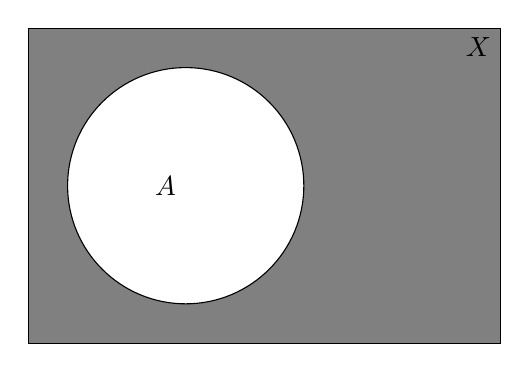
\begin{tikzpicture}
        % 全体集合の長方形を塗りつぶす
        \fill[gray] (0,0) rectangle (6,4);
        % 集合Aの円を白で塗りつぶす
        \fill[white] (2,2) circle (1.5);
        % 全体集合の枠
        \draw (0,0) rectangle (6,4) node[below left] {$X$};
        % 集合Aの円の輪郭
        \draw (2,2) circle (1.5) node[left] {$A$};
      \end{tikzpicture}
    }
    \caption{$A^c$ のベン図}
  \end{minipage}
\end{figure}


\phantomsection
\begin{example}{集合}{集合}
  例えば,$A = \{1, 2, 3\}$,$B = \{3, 4, 5\}$とすると,
  \begin{itemize*}
    \item $A \cap B = \{3\}$
    \item $A \cup B = \{1, 2, 3, 4, 5\}$
    \item $A \setminus B = \{1, 2\}$
    \item $X=\{1,2,3,4,5\}$とすると,$A^c = \{4, 5\}$
  \end{itemize*}
\end{example}

\begin{prop}{集合の交換法則}{集合の交換法則}
  $A$,$B$を集合とするとき,
  \[
    A \cap B = B \cap A , \quad A \cup B = B \cup A
  \]
  である.
\end{prop}

\begin{tleftbar}
  \begin{proof}
    共通部分および和集合の定義から従う.
  \end{proof}
\end{tleftbar}

\begin{mycolumn}
  ここで「なぜ交換法則を考えるのか」という疑問が生じるかもしれない.当たり前に成り立つことだと思える読者もいるかもしれないが,よく考えてみると「実数の減法」や「関数(写像)の合成」,「行列の積」など,
  数学において一般に交換法則が成り立たないものは数多く存在する.集合に対して交換法則を考える意義はそこにあるのである.
\end{mycolumn}

\subsubsection{集合の分配律}

\phantomsection
\begin{prop}{集合の分配律}{集合の分配律}
  $A$,$B$,$C$を集合とするとき,
  \begin{align*}
    A \cap ( B \cup C) & = (A \cap B) \cup (A \cap C), \\
    A \cup ( B \cap C) & = (A \cup B) \cap (A \cup C).
  \end{align*}
\end{prop}

\begin{tleftbar}
  \begin{proof}
    まず,
    \[
      A \cap (B \cup C) \subset (A \cap B) \cup (A \cap C)
    \]
    を示す:

    $x \in A \cap (B \cup C)$ とすると,$x$ は $A$ に属し,かつ $B \cup C$ に属する.
    すると $x \in B \cup C$ なので,$x \in B$ または $x \in C$ のいずれかが成り立つ.
    \begin{itemize}
      \item もし $x \in B$ であれば,$x$ は $A$ に属し $B$ にも属するので,$x \in A \cap B$ となる.よって $x \in (A \cap B) \cup (A \cap C)$ が従う.
      \item もし $x \in C$ であれば,$x$ は $A$ に属し $C$ にも属するので,$x \in A \cap C$ となる.よって $x \in (A \cap B) \cup (A \cap C)$ が従う.
    \end{itemize}
    いずれの場合でも $x \in (A \cap B) \cup (A \cap C)$ となるので,
    \[
      A \cap (B \cup C) \subset (A \cap B) \cup (A \cap C)
    \]
    が示された.

    次に,
    \[
      (A \cap B) \cup (A \cap C) \subset A \cap (B \cup C)
    \]
    を示す:

    $x \in (A \cap B) \cup (A \cap C)$ とすると,$x \in A \cap B$ または $x \in A \cap C$ のいずれかが成り立つ.
    \begin{itemize}
      \item もし $x \in A \cap B$ であれば,$x$ は $A$ に属し,かつ $B$ に属する.すると $B \subset B \cup C$ だから $x \in B \cup C$ でもある.よって $x \in A \cap (B \cup C)$ が成り立つ.
      \item もし $x \in A \cap C$ であれば,$x$ は $A$ に属し,かつ $C$ に属する.すると $C \subset B \cup C$ だから $x \in B \cup C$ でもある.よって $x \in A \cap (B \cup C)$ が成り立つ.
    \end{itemize}
    いずれの場合でも $x \in A \cap (B \cup C)$ となるので,
    \[
      (A \cap B) \cup (A \cap C) \subset A \cap (B \cup C)
    \]
    が示された.

    以上の2つの包含関係から,
    \[
      A \cap (B \cup C) =(A \cap B) \cup (A \cap C)
    \]
    が成り立つ.
  \end{proof}
\end{tleftbar}

\draftnote{ここに諸定理を追加予定}